\section{Theorie}
\label{sec:Theorie}
Relaxation bezeichnet in der Physik einen nicht-oszillatorischen Übergang eines Systems hin zu einem stabilen Endzustand, nachdem es aus diesem entfernt wurde.
Die Änderungsgeschwindigkeit $\dot{A}$ einer physikalischen Größe $A$ ist dabei meist proportional zur Abweichung zwischen $A$ zu einem Zeitpunkt $t$ und seinem Endzustand $A(\infty)$.
Die Integration dieses Zusammenhangs vom Zeitpunkt $0$ bis zu einem Zeitpunkt $t$ liefert:
\begin{equation}
	\label{eqn:relaxation}
	A(t)=A(\infty) + ( A(0)-A(\infty) ) \cdot e^{ct}\, ,\,\, \text{mit}\,\, c<0 .
	%
	%Hier sagt sie c definieren, keine Ahnung ob sie meint, dass c aus R ist oder was
	%c für ne physikalische Bedeutung hat...
	%
\end{equation}

Auf- und Entladevorgänge von Kondensatoren sind Beispiele für Relaxationsvorgänge und sollen im Folgenden detaillierter betrachtet werden.
\subsection{Entladevorgang eines Kondensators}
Bei einem geladenen Kondensator mit der Kapazität $C$ befindet sich die Ladung $Q$ auf den Platten.
Zwischen den Kondensatorplatten liegt dabei die Spannung $U_\text{C}$ an. Mit
\begin{equation*}
	U_\text{C}=\frac{Q}{C}
\end{equation*}
und dem Ohmschen Gesetz lässt sich $\dot{Q}=I$ zu
\begin{equation}
	\dot{Q}=-\frac{1}{RC}Q(t)
	%
	%Hier sagt sie R definieren, gleiche Frage wie oben...
	%
\end{equation}
umformen.
Da sich der Kondensator nach unendlich langer Zeit entladen wird, folgt unter Verwendung von Formel \eqref{eqn:relaxation} für den zeitlichen Verlauf der Entladung

\begin{equation}
	\label{eqn:aufladung}
	Q(t)=Q(0)(e^{-\frac{t}{RC}}) \text{.}
\end{equation}
\subsection{Aufladevorgang eines Kondensators}
Für die Aufladung des Kondensators durch eine Spannungsquelle mit $U_0$ über einen Widerstand erhält man mit ähnlichen Überlegungen unter Beachtung der Anfangsbedingungen $Q(0)=0$ und $Q(\infty)=CU_\text{0}$

\begin{equation}
	\label{eqn:entladung}
	Q(t)=CU_\text{0}(  1-e^{-\frac{t}{RC}} ) .
\end{equation}
$RC$ wird hierbei als Zeitkonstante des Systems bezeichnet.\\
\\Relaxationsvorgänge sind auch bei periodisch angeregten Systemen zu beobachten.
Liegt an einem RC-Kreis eine Wechselspannung $U(t)=U_\text{0}\cos(\omega t)$ an, und $\omega \ll \frac{1}{RC}$ gilt, ist $U_\text{C} \approx U(t)$.
Für große $\omega$ ist dies nicht mehr erfüllt, da die Amplitude von $U_\text{C}$ mit größer werdenden $\omega$ abnimmt.
\begin{figure}
	\centering
	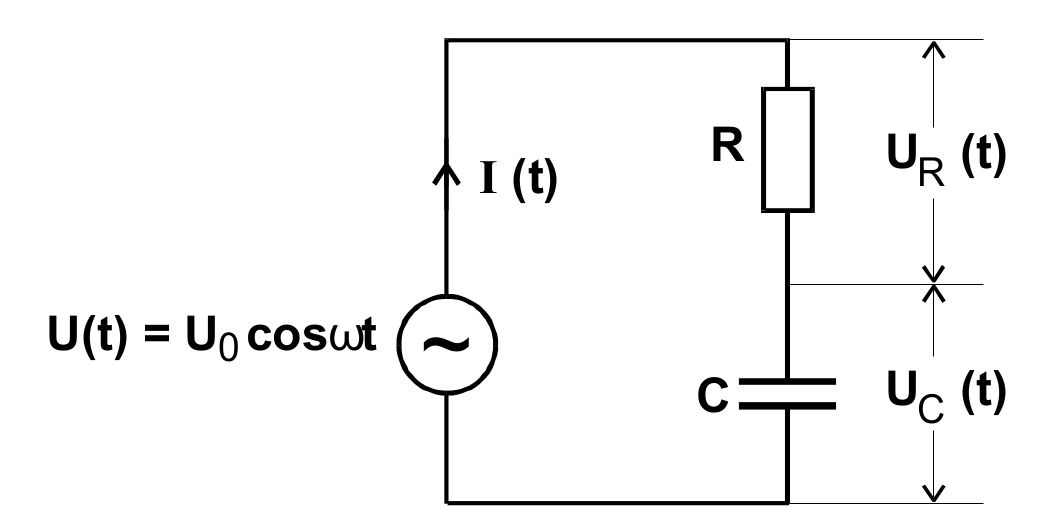
\includegraphics[width=0.7\textwidth]{bilder/periodisch.png}
	\caption{Schaltung zur Diskussion von Relaxationsvorgängen unter Einfluss von periodischer Anregung \cite{Anleitung}.}
	\label{fig:periodisch}
\end{figure}
Unter Verwendung des Ansatzes
\begin{equation*}
	U_\text{C}=A(\omega)\cos(\omega t +\phi(\omega)) ,
\end{equation*}
ergibt sich mit den Kirchhoffschen Regeln und einigen Umformungen
\begin{equation}
	\label{eqn:phase}
	\phi(\omega)=\arctan(-\omega RC) \text{.}
\end{equation}
Weitere Umformungen liefern
\begin{equation}
	\label{eqn:sinphase}
	\sin(\phi)=\frac{\omega RC}{\sqrt{1+\omega ^2R^2C^2}} \text{,}
\end{equation}
sowie
\begin{equation}
	\label{eqn:amplitude}
	A(\omega)=\frac{U_\text{0}}{\sqrt{1+\omega ^2R^2C^2}} .
\end{equation}
Für sehr kleine, beziehungsweise sehr große Frequenzen erhält man die folgenden Grenzfälle:

\begin{table*}
	\centering
	\label{tab:tab1}
	\begin{tabular}{cc}
		\toprule
		$\omega \ll \frac{1}{RC} $  & $ \omega \gg \frac{1}{RC}$ \\
		\midrule
		$\phi \to 0$                & $\phi \to \frac{\pi}{2}$   \\
		$A(\omega) \to U_\text{0} $ & $A(\omega) \to 0$          \\
		\bottomrule
	\end{tabular}
\end{table*}

Da die Kondensatorspannung $U_{\text{C}}$ für $\omega \to \infty$ gegen Null geht, kann das RC-Glied als Tiefpass verwendet werden. Große Frequenzen werden weitestgehend unterdrückt und kleine Frequenzen passieren das RC-Glied nahezu unverändert. \\
\\Für genügend große Frequenzen  $\omega$ ergibt sich aus Abbildung \ref{fig:periodisch} wiederum mit den Kirchhoffschen Regeln, dass $U_\text{C}$ klein gegen $U_{\text{R}}$ und $U$ ist, also $U(t) \approx U_\text{R}(t)$ gilt.
Mittels Umformungen erhält man
\begin{equation}
	U_\text{C}(t)=\frac{1}{RC} \int_{0}^{t} U(t') dt' \text{.}
\end{equation}
Der RC-Kreis kann also - bei hohen Frequenzen - verwendet werden,  um eine angelegte Spannung $U(t)$ zu integrieren.
